\subsection{Adeline}

\begin{frame}
\frametitle{\underline{ADA}ptive \underline{LIN}ear \underline{E}lement}

\comment{
\begin{itemize}
\item \textbf{ADA}ptive \textbf{LIN}ear \textbf{E}lement
\item Verzicht auf die Einheits-Sprungfunktion 
\item Stattdessen Nutzung linearer Aktivierungsfunktion 
\begin{itemize}
	\item wird erst einmal mit der Identiätsfunktion bestzt
\end{itemize}
\item Klassifizierungs- bzw. Entscheidungsfunktion im letzten Schritt
\begin{itemize}
	\item irrelevant für Trainingsalgorithmus
\end{itemize}
\end{itemize}
}

\begin{figure}

\includegraphics[width=.9\linewidth]{./geschichtliches/adeline/img/adeline_aufbau}
\end{figure}

\end{frame}


\begin{frame}
\frametitle{Delta-Regel}

\begin{figure}
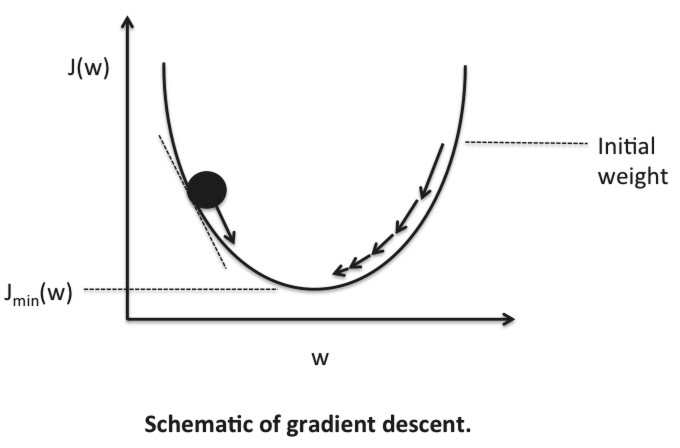
\includegraphics[width=.9\linewidth]{./geschichtliches/adeline/img/adeline_gd1_alpha}
\end{figure}

\end{frame}